%%% File encoding: UTF-8
%%% äöüÄÖÜß  <-- keine deutschen Umlaute hier? UTF-faehigen Editor verwenden!

\documentclass[foo,german]{hgbthesis}
% Zulässige Class Options:
%   Typ der Arbeit: diplom, master (default), bachelor, praktikum
%   Hauptsprache: german (default), english
%%%----------------------------------------------------------

\RequirePackage[utf8]{inputenc}		% Bei der Verw. von lualatex oder xelatex entfernen!

\graphicspath{{images/}}    % Abbildungsverzeichnis
\logofile{}				% Name des Logo-PDFs in images/ (\logofile{}, wenn kein Logo gewünscht)
\bibliography{literatur}  	% Name der Biblatex-Literaturdatei (.bib)

%%%----------------------------------------------------------
% Angaben für die Titelei (Titelseite, Erklärung etc.)
%%%----------------------------------------------------------

%%% Einträge für ALLE Arbeiten: -----------------------------
\title{Linux on z; Was unterscheidet Linux on z zu einem Linux auf x86}
\author{Timo Furrer}
\studiengang{Mainframe Topics Blockwoche}
\studienort{Hochschule Luzern}
\abgabedatum{2017}{09}{10}	% {YYYY}{MM}{DD}

%%% Zusätzlich für eine Bachelorarbeit: ---------------------
\nummer{XXXXXXXXXX-A}   % Stud-ID, z.B. 1310238045-A
% (A = 1. Bachelorarbeit)
\semester{Sommersemester 2016}
\gegenstand{Einführung in die Tiefere Problematik 1}
\betreuer{Alois B.~Treuer, Päd.\ Phil.} % oder \betreuerin{..}

%%% Restriktive Lizenformel anstatt CC (nur für Typ master) -
%\strictlicense

%%%----------------------------------------------------------
\begin{document}
%%%----------------------------------------------------------

%%%----------------------------------------------------------
\frontmatter                    % Titelei (röm. Seitenzahlen)
%%%----------------------------------------------------------

\maketitle
\tableofcontents

%\chapter{Vorwort} 	% engl. Preface


Dies ist \textbf{Version \hgbthesisDate} der \latex-Dokumentenvorlage für 
verschiedene Abschlussarbeiten an der Fakultät für Informatik, Kommunikation
und Medien der FH Oberösterreich in Hagenberg, die mittlerweile auch 
an anderen Hochschulen im In- und Ausland gerne verwendet wird.

Das Dokument entstand ursprünglich auf Anfragen von Studierenden,
nachdem im Studienjahr 2000/01 erstmals ein offizieller
\latex-Grundkurs im Studiengang Medientechnik und -design an der
FH Hagenberg angeboten wurde. Eigentlich war die Idee, die bereits
bestehende \emph{Word}-Vorlage für Diplomarbeiten "`einfach"' in
\latex\ zu übersetzen und dazu eventuell einige spezielle
Ergänzungen einzubauen. Das erwies sich rasch als wenig
zielführend, da \latex, \va was den Umgang mit Literatur und
Grafiken anbelangt, doch eine wesentlich andere Arbeitsweise
verlangt. Das Ergebnis ist -- von Grund auf neu geschrieben und
wesentlich umfangreicher als das vorherige Dokument --
letztendlich eine Anleitung für das Schreiben mit \latex, ergänzt
mit einigen speziellen (mittlerweile entfernten) Hinweisen für \emph{Word}-Benutzer.
Technische Details zur aktuellen Version finden sich in Anhang \ref{ch:TechnischeInfos}.

Während dieses Dokument anfangs ausschließlich für die Erstellung
von Diplomarbeiten gedacht war, sind nunmehr auch  
\emph{Masterarbeiten}, \emph{Bachelor\-arbeiten} und \emph{Praktikumsberichte} 
abgedeckt, wobei die Unterschiede bewusst gering gehalten wurden.

Bei der Zusammenstellung dieser Vorlage wurde versucht, mit der
Basisfunktionalität von \latex das Auslangen zu finden und -- soweit möglich --
auf zusätzliche Pakete zu verzichten. Das ist nur zum Teil gelungen;
tat\-säch\-lich ist eine Reihe von ergänzenden "`Paketen"' notwendig, wobei jedoch
nur auf gängige Erweiterungen zurückgegriffen wurde.
Selbstverständlich gibt es darüber hinaus eine Vielzahl weiterer Pakete,
die für weitere Verbesserungen und Finessen nützlich sein können. Damit kann
sich aber jeder selbst beschäftigen, sobald das notwendige Selbstvertrauen und
genügend Zeit zum Experimentieren vorhanden sind.
Eine Vielzahl von Details und Tricks sind zwar in diesem Dokument nicht explizit
angeführt, können aber im zugehörigen Quelltext jederzeit ausgeforscht
werden.

Zahlreiche KollegInnen haben durch sorgfältiges Korrekturlesen und
konstruktive Verbesserungsvorschläge wertvolle Unterstützung
geliefert. Speziell bedanken möchte ich mich bei Heinz Dobler für
die konsequente Verbesserung meines "`Computer Slangs"', bei
Elisabeth Mitterbauer für das bewährte orthographische Auge und
bei Wolfgang Hochleitner für die Tests unter Mac~OS.

Die Verwendung dieser Vorlage ist jedermann freigestellt und an
keinerlei Erwähnung gebunden. Allerdings -- wer sie als Grundlage
seiner eigenen Arbeit verwenden möchte, sollte nicht einfach
("`ung'schaut"') darauf los werken, sondern zumindest die
wichtigsten Teile des Dokuments \emph{lesen} und nach Möglichkeit
auch beherzigen. Die Erfahrung zeigt, dass dies die Qualität der
Ergebnisse deutlich zu steigern vermag.

Der Quelltext zu diesem Dokument sowie das zugehörige
\latex-Paket sind in der jeweils aktuellen Version online
verfügbar unter
%
\begin{itemize}
\item[]\url{https://sourceforge.net/projects/hgbthesis/}.
\end{itemize}
%
Trotz großer Mühe enthält dieses Dokument zweifellos Fehler und Unzulänglichkeiten
-- Kommentare, Verbesserungsvorschläge und passende Ergänzungen
sind daher stets willkommen, am einfachsten per E-Mail direkt an mich:
\begin{itemize}
\item[]%

Dr.\ Wilhelm Burger, Department für Digitale Medien,\newline
Fachhochschule Oberösterreich, Campus Hagenberg (Österreich)\newline
\nolinkurl{wilhelm.burger@fh-hagenberg.at}
\end{itemize}

\noindent
Übrigens, hier im Vorwort (das bei Diplom- und Masterarbeiten üblich, bei Bachelorarbeiten 
aber entbehrlich ist) kann kurz auf die Entstehung des Dokuments eingegangen werden.
Hier ist auch der Platz für allfällige Danksagungen (\zB an den Betreuer, 
den Begutachter, die Familie, den Hund, \ldots), Widmungen und philosophische 
Anmerkungen. Das sollte allerdings auch nicht übertrieben werden und sich auf 
einen Umfang von maximal zwei Seiten beschränken.




 % Optional. Ggf. weglassen
%\chapter{Kurzfassung}

An dieser Stelle steht eine Zusammenfassung der Arbeit, Umfang
max.\ 1 Seite. Im Unterschied zu anderen Kapiteln ist die
Kurzfassung (und das Abstract) üblicherweise nicht in Abschnitte
und Unterabschnitte gegliedert. 
Auch Fußnoten sind hier falsch am Platz.

Kurzfassungen werden übrigens häufig -- zusammen mit Autor und Titel
der Arbeit -- %
in Literaturdatenbanken aufgenommen. Es ist daher darauf zu
achten, dass die Information in der Kurzfassung für sich 
\emph{allein} (\dah ohne weitere Teile der Arbeit) zusammenhängend und
abgeschlossen ist. Insbesondere werden an dieser Stelle (wie \ua
auch im \emph{Titel} der Arbeit und im \emph{Abstract})
normalerweise \emph{keine Literaturverweise} verwendet! Falls
unbedingt solche benötigt werden -- etwa weil die Arbeit eine
Weiterentwicklung einer bestimmten, früheren Arbeit darstellt --,
dann sind \emph{vollständige} Quellenangaben in der Kurzfassung
selbst notwendig, \zB %
[\textsc{Zobel} J.: \textit{Writing for Computer Science -- The Art of
Effective Commu\-nica\-tion}. Springer-Verlag, Singa\-pur, 1997].

Auch sollte daran gedacht werden, dass bei der Aufnahme in Datenbanken
Sonderzeichen oder etwa Aufzählungen mit "`Knödellisten"' in der
Regel verloren gehen. Dasselbe gilt natürlich auch für das 
\emph{Abstract}.


Inhaltlich sollte die Kurzfassung \emph{keine} Auflistung der
einzelnen Kapitel sein (dafür ist das Einleitungskapitel
vorgesehen), sondern dem Leser einen kompakten, inhaltlichen
Überblick über die gesamte Arbeit verschaffen. Der hier verwendete
Aufbau ist daher zwangsläufig anders als der in der Einleitung.

%\chapter{Abstract}

\begin{english} %switch to English language rules
This should be a 1-page (maximum) summary of your work in English.
%und hier geht dann das Abstract weiter...
\end{english}

Im englischen Abstract sollte inhaltlich das Gleiche
stehen wie in der deutschen Kurzfassung. Versuchen Sie daher, die
Kurzfassung prä\-zise umzusetzen, ohne aber dabei Wort für Wort zu
übersetzen. Beachten Sie bei der Übersetzung, dass gewisse
Redewendungen aus dem Deutschen im Englischen kein Pendant haben
oder völlig anders formuliert werden müssen und dass die
Satzstellung im Englischen sich (bekanntlich) vom Deutschen stark
unterscheidet (mehr dazu in Abschn.\ \ref{sec:englisch}). Es
empfiehlt sich übrigens -- auch bei höchstem Vertrauen in die
persönlichen Englischkenntnisse -- eine kundige Person für das
"`proof reading"' zu engagieren.

Die richtige Übersetzung für "`Diplomarbeit"' ist übrigens
schlicht \emph{thesis}, allenfalls  "`diploma thesis"' oder "`Master's thesis"', 
auf keinen Fall aber "`diploma work"' oder gar "`dissertation"'. 
Für "`Bachelorarbeit"' ist wohl "`Bachelor thesis"' die passende Übersetzung. 

Übrigens sollte für diesen Abschnitt die \emph{Spracheinstellung} in \latex\ von Deutsch
auf Englisch umgeschaltet werden, um die richtige Form der
Silbentrennung zu erhalten, die richtigen Anführungszeichen müssen allerdings selbst gesetzt werden %
(s.\ dazu die Abschnitte \ref{sec:sprachumschaltung} %
und \ref{sec:anfuehrungszeichen}).


%%%----------------------------------------------------------
\mainmatter          % Hauptteil (ab hier arab. Seitenzahlen)
%%%----------------------------------------------------------

\chapter{Einleitung}
\label{cha:Einleitung}

\section{Was ist Linux?}

Unter dem Begriff Linux versteht man allgemein einen Ueberbegriff fuer freie Betriebssysteme, welche auf dem Linux Kernel basieren. Der Linux Kernel wurde erstmals im frühjahr 1992 unter der GNU GPL Lizenz fuer Intels x86 Architektur veroeffentlicht.

Ein konkretes Linux Betriebssystem bezeichnet man als Linux Distribution. Eine Distribution besteht aus einem Linux Kernel, GNU Tools und Libraries, zusaetzlicher Software und manchmal auch einem Window System, einem Windows Manager und einem Desktop Environment. Beispiele fuer solche Linux Distributionen sind Debian, Ubuntu, Arch Linux, openSUSE, Fedora und Linux on z.

\section{Linux Kernel Architekturen}

Der Linux Kernel ist von monolithischer aber auch modularer Natur. Dies bedeutet, dass Funktionalitaeten, welche der Kernel zwingend braucht, direkt eingebaut sind - Funktionalitaeten welche aber nur bei ganz bestimmten Hardwarekomponenten gebraucht werden, koennen ueber sogenannte Kernel Module nachgeladen werden.
Der Linux Kernel uebernimmt Aufgaben wie beispielsweise die Speicher- und Prozessverwaltung, Interprozesskommunikation, Geraeteverwaltung und Dateisystem.
Nachfolgende Grafik zeigt eine Uebersicht wichtiger Aufgaben des Linux Kernels im Zusammenspiel mit Hardware und den Userspace Anwendungen der Distribution:

\begin{figure}[h!]
\centering
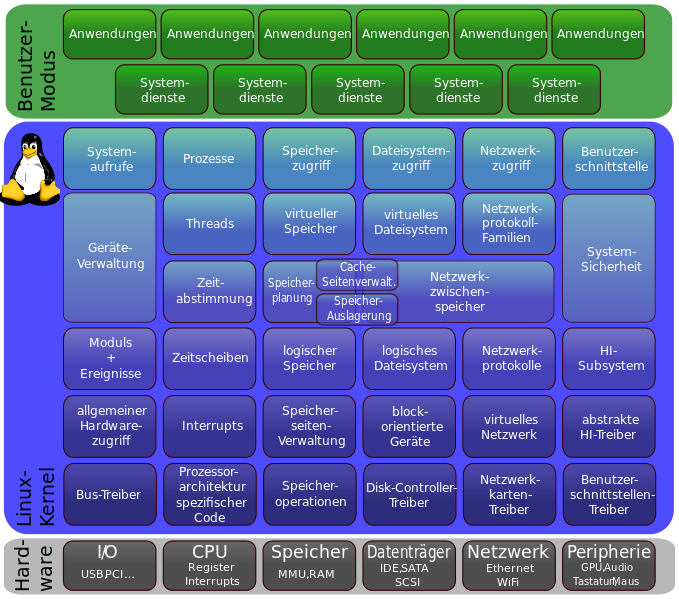
\includegraphics[width=.80\textwidth]{einleitung-kernel-struktur}
\caption{Linux Kernel Struktur\cite{KernelStruktur}.}
\label{fig:KernelStruktur}
\end{figure}

\newpage

Dieser modular-monolithischer Ansatz des Linux Kernels traegt nicht zuletzt zu seiner grossen Verbreitung auf unterschiedlichsten Architekturen und Plattformen bei.

Wikipedia fuehrt eine Liste der Computer Architekturen, welche Linux unterstuetzt.
Inzwischen sind dort ueber 100 Architekturen zu finden. Diese breite Abdeckung von Architekturen macht es moeglich, dass Linux in beinahe alle Bereiche von Betriebssystem Umgebungen Einzug gefunden hat. Diese reicht von exotischen Umgebungen, wie Navigations- und Haushaltsgeraeten, Digitalkameras, ueber Desktop- und Laptop Computern und Mobiltelefonen mit Android, bis hin zu Supercomputern und High Performance Computing Clusters mit Rocks Cluster Distribution.

So hat Linux auch seine Daseinsberechtigung auf dem Mainframe gefunden mit Linux on z, welches auf IBMs z Systems und IBMs LinuxONE laeuft.

\chapter{Linux als Kernel und Distro}
\label{cha:Linux}

\section{Was ist Linux?}

Unter dem Begriff Linux versteht man allgemein einen Überbegriff für freie Betriebssysteme, welche auf dem Linux Kernel basieren.\cite{LinuxWiki}
Der Linux Kernel wurde erstmals im Frühjahr 1992 unter der GNU GPL Lizenz für Intels x86 Architektur veröffentlicht.

Ein konkretes Linux Betriebssystem bezeichnet man als \textit{Linux Distribution} oder kurz Linux \textit{Distro}.
Eine Distribution besteht aus einem Linux Kernel, GNU Tools und Libraries, zusätzlicher Distro-spezifischer Software und manchmal auch einem Window System, einem Window Manager und einem Desktop Environment. Beispiele für solche Linux Distributionen sind Debian, Ubuntu, Arch Linux, openSUSE, Fedora und Linux on z.\cite{LinuxDistroWiki}

\section{Linux Kernel Architekturen}

Der Linux Kernel ist von monolithischer aber auch modularer Natur. Dies bedeutet, dass Funktionalität, welche der Kernel zwingend braucht, direkt eingebaut sind -- Funktionalitäten, welche aber nur bei ganz bestimmten Hardwarekomponenten gebraucht werden, können über sogenannte Kernel Module nachinstalliert und nachgeladen werden.
Der Linux Kernel übernimmt Aufgaben wie beispielsweise die Speicher- und Prozessverwaltung, Interprozesskommunikation, Geräte Verwaltung und Dateisysteme.
Nachfolgende Grafik zeigt eine Übersicht wichtiger Aufgaben des Linux Kernels im Zusammenspiel mit Hardware und den Userspace Anwendungen der Distribution:

\begin{figure}[h!]
\centering
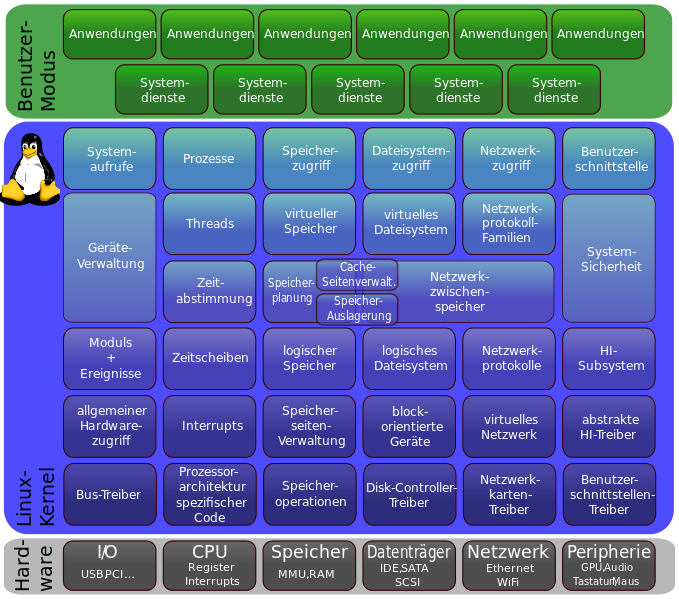
\includegraphics[width=.80\textwidth]{einleitung-kernel-struktur}
\caption{Linux Kernel Struktur\cite{KernelStruktur}.}
\label{fig:KernelStruktur}
\end{figure}

\newpage

Dieser modular-monolithischer Ansatz des Linux Kernels trägt nicht zuletzt zu seiner grossen Verbreitung auf unterschiedlichsten Architekturen und Plattformen bei.

Wikipedia führt eine Liste der Computer Architekturen, welche Linux unterstützt.\footnote{Siehe \url{https://en.wikipedia.org/wiki/List_of_Linux-supported_computer_architectures}}
Inzwischen sind dort über 100 Architekturen zu finden. Diese breite Abdeckung von Architekturen macht es möglich, dass Linux in beinahe alle Bereiche von Betriebssystem Umgebungen Einzug gefunden hat. Diese reicht von exotischen Umgebungen, wie Navigations- und Haushaltsgeräten, Digitalkameras, über Desktop- und Laptop Computern und Mobiltelefonen mit Android, bis hin zu Supercomputern und High Performance Computing Clusters mit Rocks Cluster Distribution.

So hat Linux auch seine Daseinsberechtigung auf dem Mainframe gefunden mit Linux on z, welches auf IBMs z Systems und IBMs LinuxONE läuft.

%\chapter{Linux unter x86}
\label{cha:Linux_x86}

Die x86 Architektur war die erste unterstuetze Architektur im Linux Kernel. Dies aus dem einfachen Grund, dass Linus Torvalds, Author und Maintainer von Linux, den Linux Kernel fuer seinen persoenlichen Rechner entwickelt hat, welcher eine Intel x86 CPU hatte.

Von Beginn an wurde x86 vom Linux Kernel unterstuetzt. Auch Support fuer 64-Bit Architekturen liessen nicht lange auf sich warten.

\section{Hauptmerkmale}

\section{Ziel Plattform}

\section{Eigenschaften}

\chapter{Linux on z}
\label{cha:Linux_on_z}

“Linux on z” ist ein Sammelbegriff fuer Linux Distributionen welche auf einem IBM Mainframe laufen wie beispielsweise auf den IBM z Systems und den IBM LinuxONE Servern.

Im Jahr 1999 hat IBM mehrere Patches, welche hauptsaehlich aus “object code only” (OCO) Modulen bestanden, fuer den damals aktuellen Linux Kernel 2.2.13 veroeffentlicht.
Ungefaehr ein Jahr spaeter hat IBM diese OCO Module durch Open Source Module im Kernel ersetzt und Linux on z formal als IBM Produkt vorgestellt.

\section{Integrated Facility for Linux (IFL)}

In einer IBM Mainframe Umgebung werden dem Kunden pro Taktzyklus von einem General Purpose Processor (CP) Nutzungsgebuehren berechnet. Um diese Nutzungskosten zu senken hat IBM drei spezielle Arten von Prozessoren entwickelt:
zAAP fuer Java Code
zIIP fuer DB2
IFL um Linux laufen zu lassen
Der IFL ist hardware-technisch nichts anderes als ein standard CP mit dem Unterschied, dass der Microcode die CP auf Linux und z/VM Instruktionen beschraenkt.

\section{Hauptmerkmale von Linux on z}

Das Ziel von Linux on z ist es die Vorteile eines IBM Mainframes mit einem Linux Betriebssystems zu nutzen, sodass Linux seine Charakteristiken behalten kann.

Das “Look \& Feel” von Linux on z soll dem entsprechen, was sich ein erfahrener Linux User gewohnt ist. Dazu gehoeren unter anderem:

Linux als ASCII Environment
Konform zum Linux Standard Base (LSB) und zum Filesystem Hierarchy Standard (FHS)
Kompatibel mit POSIX
Kein eigener Linux Kernel Fork fuer Linux on z - Mainline.

Die folgende Grafik zeigt, welche Linux- und GNU toolchain-Komponenten kleine Codeaenderungen zu Nutze machen:

\begin{figure}[h!]
\centering
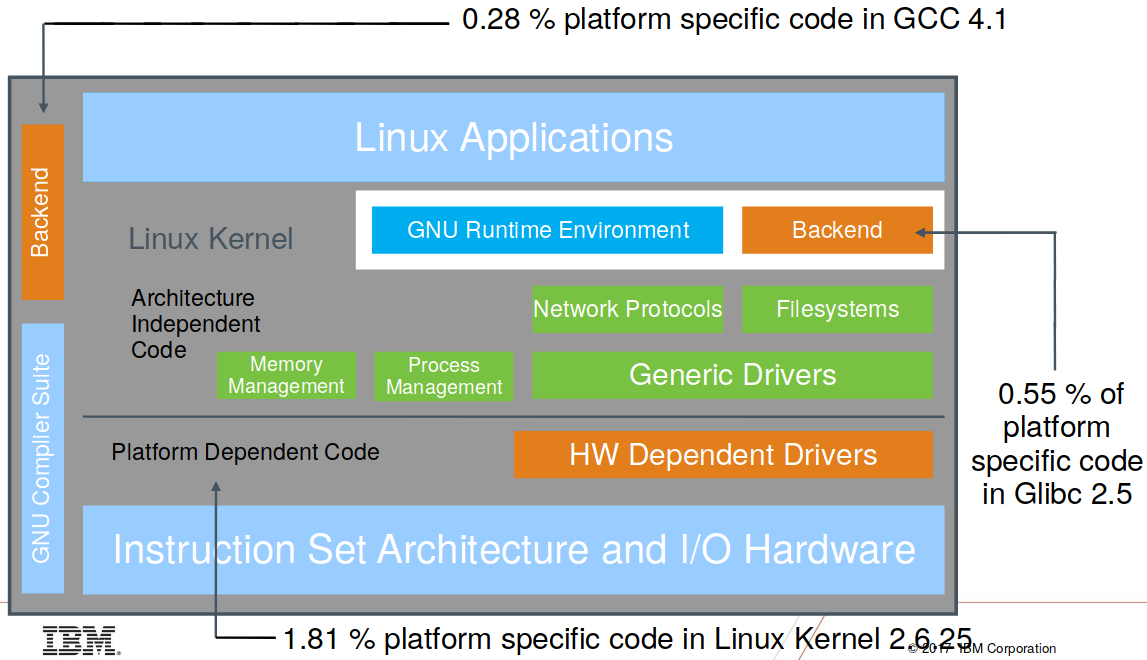
\includegraphics[width=.95\textwidth]{linux-on-z-kernel-struktur.png}
\caption{Linux on z Kernel\cite{LinuxOnZKernel}.}
\label{fig:LinuxOnZKernel}
\end{figure}

Wie man von der Grafik entnehmen kann, war dies der Stand des bereits fast 10 Jahre alten Linux Kernels 2.6.25.

\section{IBM Mainframe Eigenschaften fuer Linux}

Wie schon im letzten Kapitel angeschnitten, ist ein grosses Ziel von Linux on z die Vorteile eines IBM Mainframes fuer Linux nutzen zu koennen.

IBM macht mit Linux on z folgende Angebote fuer Linux nutzbar:

\begin{figure}[h!]
\centering
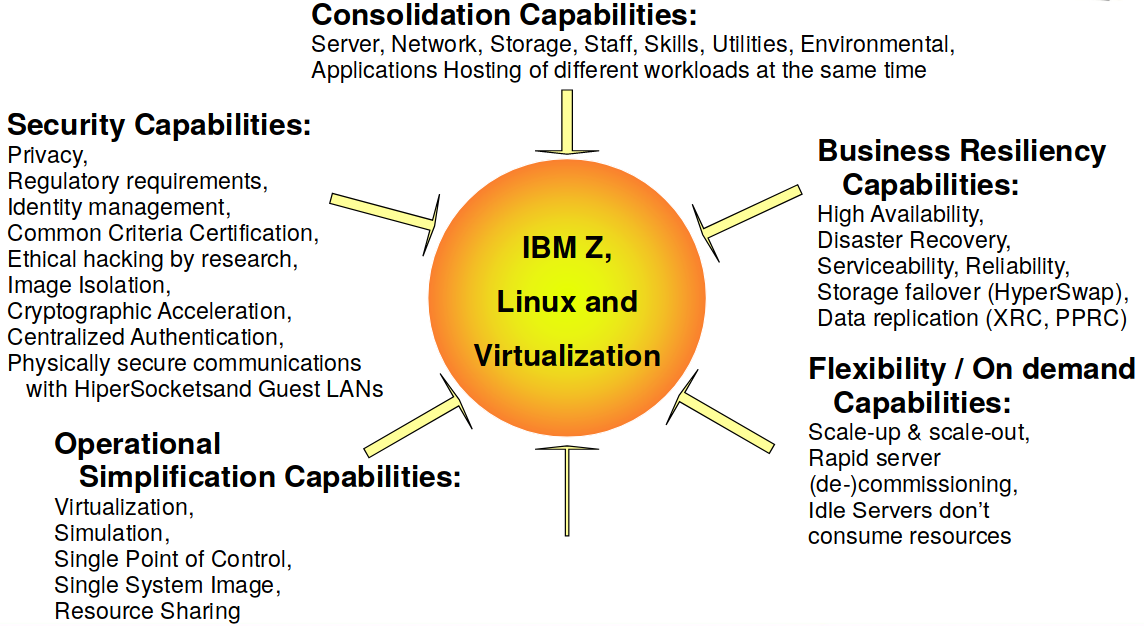
\includegraphics[width=.80\textwidth]{linux-on-z-mainframe-vorteile.png}
\caption{Linux on z Mainframe Vorteile\cite{LinuxOnZMainframeVorteile}.}
\label{fig:LinuxOnZMainframeVorteile}
\end{figure}

\section{Ziel Plattformen}

Linux on z kann auf zwei verschiedene Arten auf einem Mainframe laufen: in LPARs oder als virtuelle Maschine unter z/VM. Aeltere Linux on z, welche noch fuer S/390 31-Bit Hardware entwickelt wurden, konnten auch direkt ohne Virtualisierung auf einem Mainframe laufen.
Fuer aktuelle 64-Bit S/390x Linux on z ist dies nicht mehr moeglich.

\subsection{Linux on z in LPARs}

Linux on z kann auf einem oder mehreren Logical Partitions (LPARs) installiert und laufen gelassen werden. Aktuelle z13 und z14 Mainframes unterstuetzen bis zu 85 LPARs - es koennten also theoretisch 85 Linux on z Instanzen auf einem einzigen Mainframe laufen, ohne dass VMs zum Einsatz kommen.
Es ist auch moeglich nur auf einem Teil der LPARs Linux zu installieren und auf anderen LPARs ein anderes Mainframe Betriebssystem, wie z.B. z/OS:

\begin{figure}[h!]
\centering
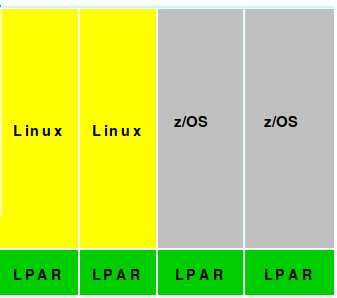
\includegraphics[width=.75\textwidth]{linux-on-z-linux-on-lpar.png}
\caption{Linux on z in LPARs\cite{LinuxOnZOnLPAR}.}
\label{fig:LinuxOnZOnLPAR}
\end{figure}

\subsection{Linux on z in z/VM}

Die zweite Moeglichkeit wie Linux on z auf einem Mainframe laufen gelassen werden kann, ist mit Hilfe einer Virtualisierung durch z/VM. Dabei wird Linux on z in einer full-virtualized Virtuelle Maschinen betrieben. z/VM wird in dieser Varianten selbst auch in eine LPAR installiert:

\begin{figure}[h!]
\centering
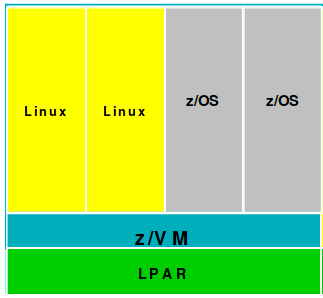
\includegraphics[width=.75\textwidth]{linux-on-z-linux-on-zvm.png}
\caption{Linux on z unter z/VM\cite{LinuxOnZOnZVM}.}
\label{fig:LinuxOnZOnZVM}
\end{figure}

\subsection{Linux on z: LPAR oder z/VM?}

Bei der Entscheidung ob Linux on z in einer LPAR oder unter z/VM installiert werden soll, spielen viele Faktoren eine Rolle:

Anzahl der gewuenschten Linux Instanzen
Kommunikation zwischen verschiedenen Instanzen
Muessen andere Server auf dem gleichen Mainframe laufen
Flexibilitaet -> + z/VM

Es ist auch moeglich LPARs und z/VM Linux on z Instanzen auf einem Mainframe zu mischen:

\begin{figure}[ht!]
\centering
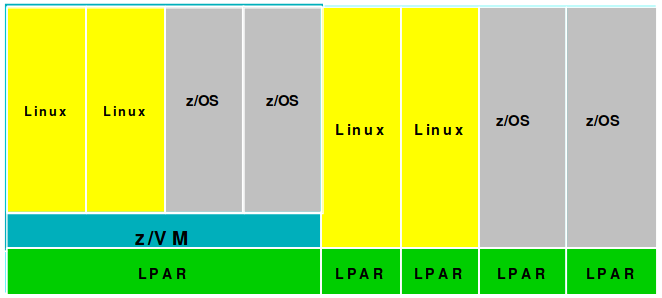
\includegraphics[width=.75\textwidth]{linux-on-z-linux-on-lpar-zvm.png}
\caption{Linux on z in LPARs und unter z/VM\cite{LinuxOnZOnLPARZVM}.}
\label{fig:LinuxOnZOnLPARZVM}
\end{figure}

\chapter{Linux auf x86 vs. z Systems}
\label{cha:Unterschiede}

In den folgenden Abschnitten werden einige wichtige Unterschiede zwischen einem Linux für x86 und Linux on z behandelt.

\section{Workload Management}
\label{sec:WorkloadManagement}

Die IBM z Systems haben ein nahezu perfektes Workload Management.
Mit Linux on z wird auf einem Mainframe von ziemlich simplen Konzepten Gebrauch gemacht, um den Workload zu optimieren
und zwischen High- und Low- Priority Workload zu unterscheiden:\cite{IBMRedBookWorkloadConcept}

\begin{description}
    \item[Identifizieren des Workloads]{Es muss identifiziert werden, was die laufenden Workloads sind.}
    \item[Messen wie lange diese Workloads dauern]{Es muss gemessen werden, wie lange diese Workloads dauern.}
    \item[Ausfindig machen der Uebergabe Punkten]{Wenn man herausgefunden hat, was die Workloads sind und wie lange diese dauern, kann begonnen werden die Last zu optimieren.}
\end{description}

\newpage
Diese Workload Management Konzepte führen dazu, dass mit Linux on z die volle Prozessleistung genutzt werden kann (high utilitzation).

\begin{figure}[h!]
\centering
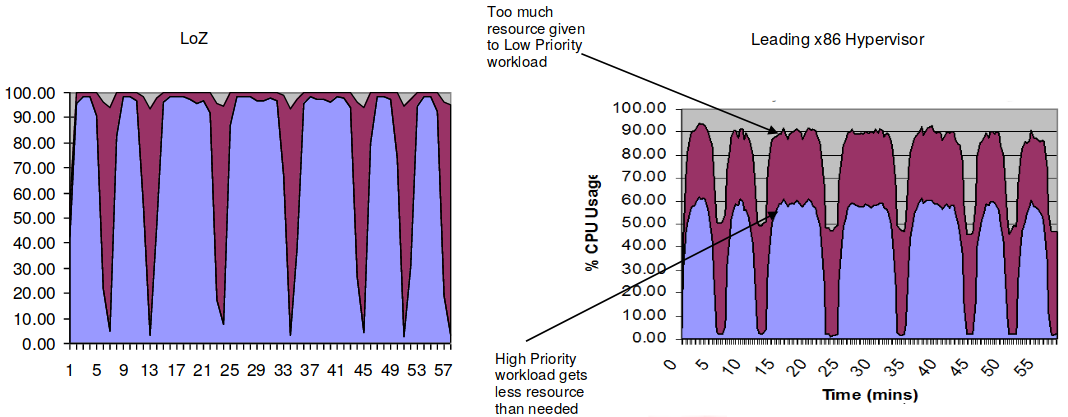
\includegraphics[width=.95\textwidth]{difference-workload-management}
\caption{Workload Management Vergleich mit x86\cite{WorkloadManagement}.}
\label{fig:WorkloadManagement}
\end{figure}

\section{Konsolidierung von Linux Servern}
\label{sec:Konsolidierung}

In Rechenzentren hat man oft das Ziel, die Unterhaltungskosten und Effizienz zu optimieren.
Nicht nur was Platz und Strom angeht sondern auch die Effizienz und Auslastung der Server.
Ein IBM Mainframe mit Linux on z ist prädestiniert dafür komplette Linux Server Farmen auf einer
einzelnen Hardware zu konsolidieren.
Damit es sich überhaupt lohnt eine solche Konsolidierung in Betracht zu ziehen, braucht man eine kritische Masse
an Linux Servern. IBM illustriert diese \textit{kritische Masse} wie folgt:

\begin{figure}[h!]
\centering
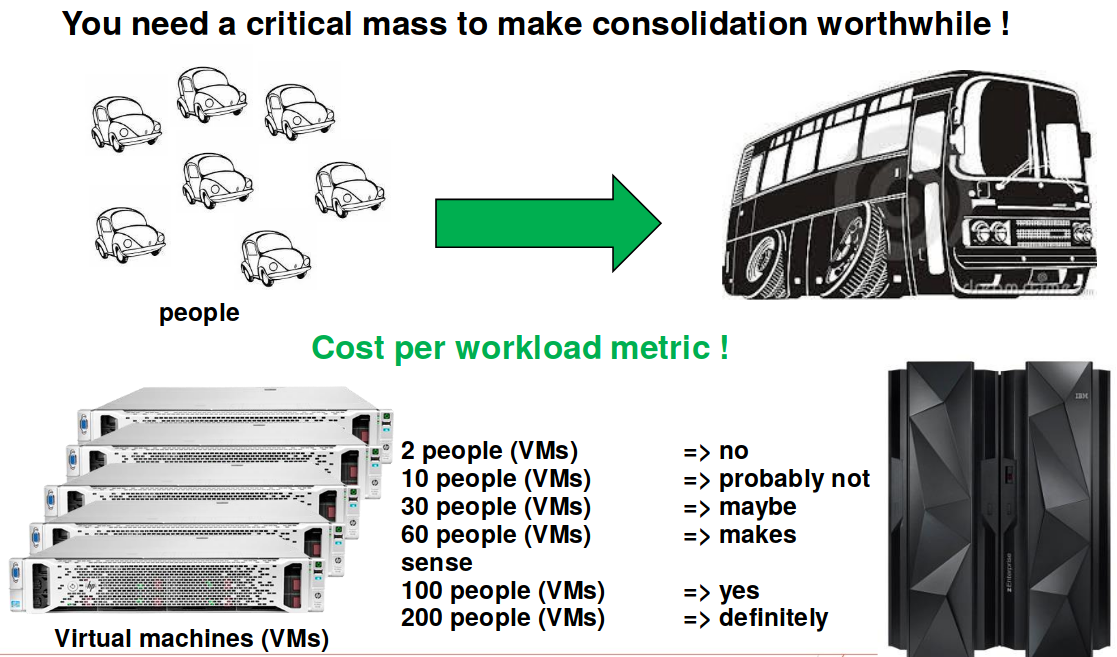
\includegraphics[width=.80\textwidth]{difference-kritische-masse}
\caption{Kritische Masse fuer Konsolidierung\cite{KonsolidierungKritischeMasse}.}
\label{fig:KonsolidierungKritischeMasse}
\end{figure}

IBM hat laut mehreren \textit{Eagle studies} folgende Statistik aufgestellt im Bezug auf x86-Cores zu Linux on z-Cores:

\begin{figure}[h!]
\centering
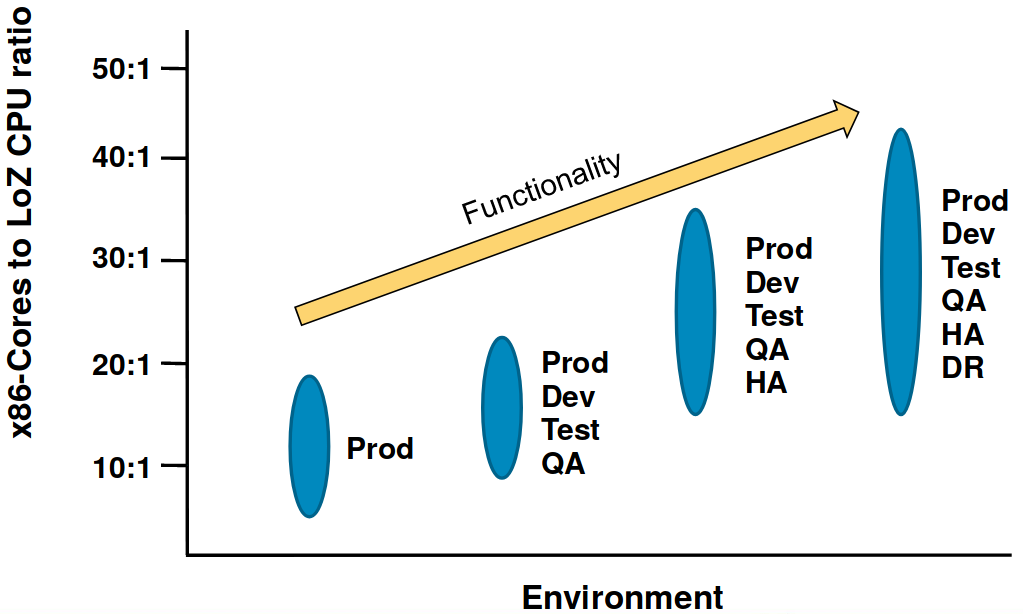
\includegraphics[width=.80\textwidth]{difference-cpu-ratio}
\caption{Rate von x86-Cores zu LoZ-Cores\cite{CPURatio}.}
\label{fig:CPURatio}
\end{figure}

Diese Statistik zeigt, dass umso komplexer ein Environment wird, umso mehr x86-Cores werden im Vergleich zu Linux on z-Cores gebraucht,
damit das Environment die erforderlichen Leistungen erbringen kann.

Dies ist vor allem auf die gute Leistung des Workload Managements zurückzuführen.\footnote{Siehe Abschnitt \ref{sec:WorkloadManagement}}

\section{Kommunikation ueber HiperSockets}
\label{sec:HiperSockets}

Wenn man Applikationssysteme mit mehreren verschiedenen physikalisch getrennten x86 Servern hat, so wird die Kommunikation zwischen diesen meist über Switches mit TCP/IP geroutet. Das Problem dabei ist die Latenzzeit dieser Netzwerkverbindung.
Vor allem bei Systemen bestehend aus Microservices\footnote{man hat also viele kleinere Systeme welche kleine Teilaufgaben einer grösseren Aufgabe übernehmen} kann die Latenzzeit zwischen den Services einen beachtlichen Anteil der gesamt Rechenzeit ausmachen.

Die IBM Mainframes bieten diesen Latenzzeiten mit sogenannten HiperSockets Abhilfe.\cite{HiperSocketsWiki}
HiperSockets bieten \textit{high-speed} \textit{in-memory} TCP/IP Kommunikationskanäle zwischen verschiedenen LPARs an. IBM unterstützt HiperSockets für z/OS, z/VM und auch für Linux on z.

HiperSockets sind ein starkes Argument für die Konsolidierung von x86 Servern auf ein Mainframe. Nicht nur fallen die Kosten für Switches und Kabel nicht sondern es kommt auch noch ein riesen Performance-Vorteil hinzu.

\subsection{HiperSockets als Address-Family}

Der Linux Kernel unterstützt mit der \textit{AF\_IUCV} Address Family eine direkte Kommunikation über HiperSockets zwischen Applikationen laufend auf verschiedenen Linux on z Instanzen.
Für Linux on z in LPARs werden folgende Funktionalitäten unterstützt:
\begin{itemize}
    \item{Mehrere eingehenden \textit{echte} HiperSocket Verbindungen}
    \item{Mehrere ausgehende \textit{echte} HiperSocket Verbindungen}
\end{itemize}
Wird Linux on z unter z/VM betrieben kommen IUCV-Verbinunden\footnote{IUCV steht für Inter-User Communication Vehicle und wird gebraucht, damit mehrere z/VM und Applikationen unter z/VM miteinander kommunizieren können} und keine \textit{echte} HiperSockets zum Einsatz.

Der \textit{AF\_IUCV} Support kann im Linux Kernel über die \textit{CONFIG\_IUCV} und \textit{CONFIG\_AFIUCV} Optionen aktiviert werden.

\begin{figure}[h!]
\centering
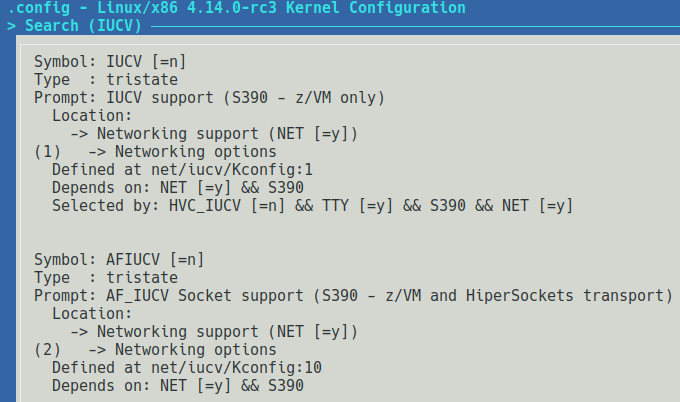
\includegraphics[width=.80\textwidth]{afiucv_menuconfig}
\caption{Linux Kernel \textit{menuconfig} AF\textunderscore IUCV Optionen}
\label{fig:AFIUCVMENUCONFIG}
\end{figure}

Wie bei fast allen Modulen kann der \textit{AF\_IUCV} entweder direkt in den Kernel einkompiliert oder als dynamisches Modul nachgeladen werden.
Das nachladbare Modul heisst \textit{af\_iucv}:\cite{IBMAFIUCV}

\begin{lstlisting}
# modprobe af_iucv
\end{lstlisting}

\section{Call Home - Problem Reporting}

IBM bietet ein Linux Kernel Modul an um, im Falle einer Kernel Panic\footnote{Ein Crash im Kernelspace}, direkt Problem Reports an RETAIN -- ein Datenbank System um die IBM Fieldagents und Kunden zu unterstützen -- zu senden.

Um diese automatischen Problem Reports zu nutzen, müssen folgende Anforderungen erfüllt sein:\cite{IBMCallHome}
\begin{itemize}
    \item{Linux on z muss direkt in einer LPAR installiert sein}
    \item{Der Linux Kernel muss das \textit{SCLP\_ASYNC} device unterstützen}
    \item{Der Kunde braucht ein \textit{Hardware support agreement} mit IBM um die Reports an RETAIN schicken zu dürfen}
\end{itemize}

\subsection{Kernel Konfiguration}

Damit die \textit{Call Home} Funktionalitaet auf Linux Kernel Ebene funktioniert muss die \textit{CONFIG\_SCLP\_ASYNC} Option im Kernel aktiviert sein.

\begin{figure}[h!]
\centering
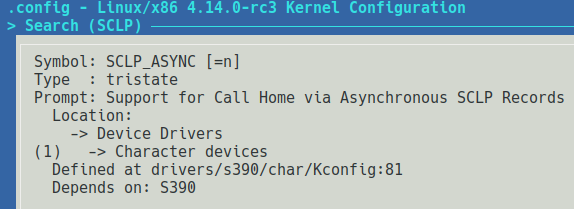
\includegraphics[width=.80\textwidth]{sclp_async_menuconfig}
\caption{Linux Kernel \textit{menuconfig} SCLP\textunderscore ASYNC Optionen}
\label{fig:SCLPASYNC}
\end{figure}

\textit{SCLP\_ASYNC} funktioniert sowohl direkt im Kernel als auch als nachladbares Kernel Module \textit{sclp\_async}:

\begin{lstlisting}
# modprobe sclp_async
\end{lstlisting}

Sobald das Kernel Modul aktiv ist, kann die \textit{Call Home} Funktion übers \textit{procfs} eingeschalten oder wieder ausgeschalten werden:\cite{IBMCallHome}

\begin{lstlisting}
# # Enable call home support
# echo 1 > /proc/sys/kernel/callhome
# # Disable call home support
# echo 0 > /rpco/sys/kernel/callhome
\end{lstlisting}

\section{Ecosystem}

Wie schon im Linux unter x86 Abschnitt\footnote{Siehe Abschnitt \ref{sec:LinuxOnx86}} kurz erwähnt wurde, hat die x86 Architektur, über die Jahre hinweg, ein ungeschlagenes Ecosystem aufbauen können.
Damit sind nicht nur die vielen Hersteller von x86 Architekturen gemeint, sondern auch die vielen Distributionen und Applikationen die für x86 veröffentlicht werden.\cite{x86Manufacturer}

Für eine Firma können die Kosten und der Aufwand, ein grosses business-kritisches System von x86 auf s390x zu portieren, schlicht und einfach zu gross sein.

\subsection{x86 Applikation unter Linux on z}

Dem will IBM mit \textit{x86 proxy processes} Abhilfe schaffen.
Diese Proxy Prozesse laufen, wie normale Prozesse, auf einem Linux on z und repräsentieren eine x86 Applikation inklusive deren Lebenszyklus und Ressourcen.
Diese x86 Applikation und deren eigentliche Prozesse laufen dabei nicht direkt auf dem selben Linux on z, sondern weiterhin auf einem normalen x86 Server:

\begin{figure}[h!]
\centering
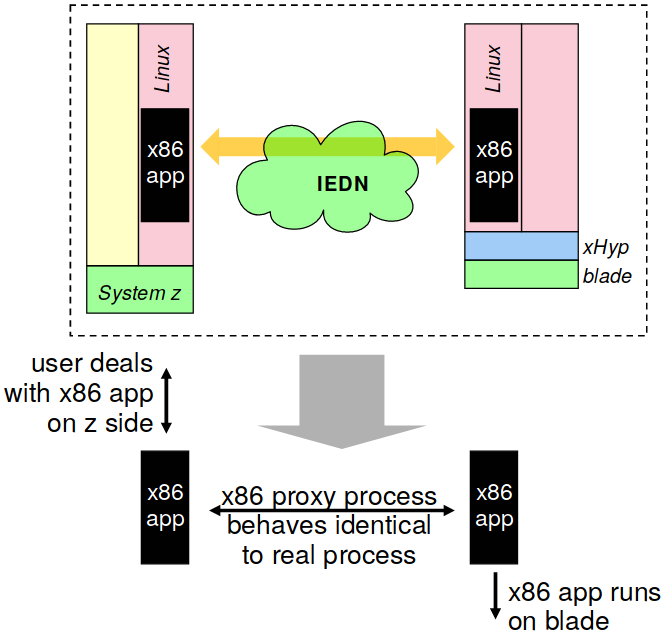
\includegraphics[width=.80\textwidth]{difference-integrated}
\caption{x86 Applikation integriert in Linux on z\cite{x86OnLinuxOnZ}.}
\label{fig:LinuxOnZ}
\end{figure}

Die x86 Applikation kann damit nahtlos in ein Linux on z fast integriert werden und so die Konsolidierung einer Serverumgebung schrittweise ermöglichen.\cite{x86OnLinuxOnZ}

\chapter{Fazit}
\label{cha:Schluss}

Auch wenn diese Arbeit das Aufarbeiten von nur wenigen Unterschieden zwischen Linux on x86 und Linux on z zugelassen hat, so haben die vorgängigen Kapitel gezeigt, dass es durchaus Sinn machen kann grössere Linux x86 Server Infrastrukturen auf ein Mainframe mit Linux on z zu konsolidieren.
Ich denke die Hauptgründe dafür sind:
\begin{description}
    \item[Eine Hardware]{Eine Mainframe Hardware ist in der Lage hunderte Linux on z Instanzen laufen zu lassen. Der Footprint eines IBM Mainframes erspart Platz, Strom und im Endeffekt dann vor allem auch Geld.\footnote{Siehe Abschnitt \ref{sec:Konsolidierung}}}
    \item[Workload Management]{Da die Linux on z Instanzen auf einer einzigen grossen Hardware laufen, hat ein Mainframe die Möglichkeit den Workload perfekt auf die zur Verfügung stehenden Ressourcen zu verteilen.\footnote{Siehe Abschnitt \ref{sec:WorkloadManagement}}}
    \item[Exterm performante Kommunikation]{Mit HiperSockets bietet Linux on z eine extrem performante \textit{in-memory} TCP/IP Kommunikationsschnittstelle\footnote{Siehe Abschnitt \ref{sec:HiperSockets}}}
    \item[Call Home]{Die Call Home Funktion im Linux Kernel vereinfacht das Raportieren von Kernel Panics an IBM.}
\end{description}


%%%----------------------------------------------------------
\appendix                                            % Anhang
%%%----------------------------------------------------------

%%%----------------------------------------------------------
\MakeBibliography                        % Quellenverzeichnis
\listoffigures                           % Abbildungsverzeichnis
%%%----------------------------------------------------------

%%% Messbox zur Druckkontrolle ------------------------------
\chapter*{Messbox zur Druckkontrolle}



\begin{center}
{\Large --- Druckgröße kontrollieren! ---}

\bigskip

\Messbox{100}{50} % Angabe der Breite/Hoehe in mm

\bigskip

{\Large --- Diese Seite nach dem Druck entfernen! ---}

\end{center}



%%%----------------------------------------------------------
\end{document}
%%%----------------------------------------------------------
